\section{Introduction to Machine Learning}
    Machine learning is a subset of artificial intelligence that focuses on developing algorithms and statistical models that enable computers to learn from and make predictions based on data. 
    It is used in a wide range of applications, including image and speech recognition, medical diagnosis, and financial forecasting. 
    Machine learning can be broadly categorized into three types: supervised learning, unsupervised learning, and reinforcement learning.

    Machine learning is useful for tasks where it is difficult to explicitly program the rules or patterns, such as recognizing handwritten digits or detecting spam emails.

    By training a model on a dataset, the model can learn the underlying patterns and relationships in the data and make predictions on new, unseen data.

\section{Structure of Neural Networks}
    Neural networks are a class of machine learning models inspired by the structure and function of the human brain. They consist of interconnected nodes, or neurons, organized in layers. Each neuron receives input, processes it, and produces an output that is passed to the next layer. The connections between neurons are represented by weights, which are learned during the training process.

    \vspace{1em} \noindent The basic building block of a neural network is the perceptron, which takes a set of inputs, applies weights to them, and passes the weighted sum through an activation function to produce an output. Multiple perceptrons are connected in layers to form a neural network. The most common type of neural network is the feedforward neural network, where information flows in one direction from the input layer to the output layer.

    \vspace{1em} \noindent Neural networks can have multiple layers, with each layer performing a different transformation on the input data. The input layer receives the input data, the hidden layers process the data, and the output layer produces the final output. The number of layers and the number of neurons in each layer are hyperparameters that can be tuned to optimize the performance of the network.

    \begin{figure}[h]
        \centering
        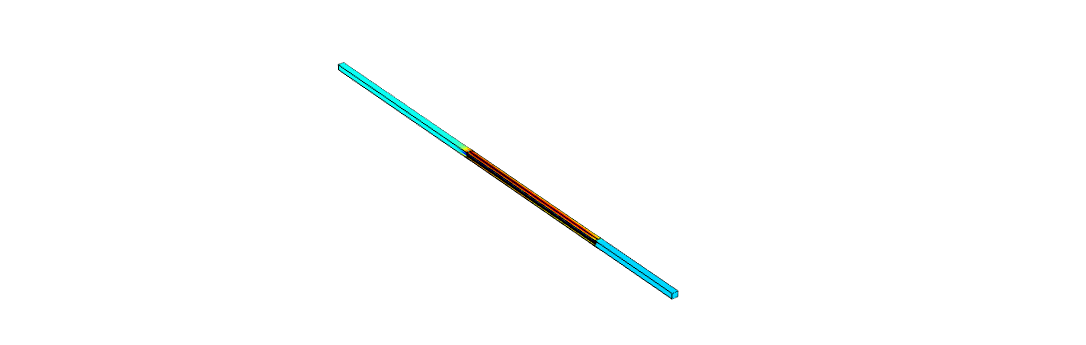
\includegraphics[width=0.8\textwidth]{00_Images/00_Velocity.png}
        \caption{Structure of a feedforward neural network.}
        \label{fig:neural_network}
    \end{figure}

    \subsection{Types of Layers}
        \noindent Neural networks have multiple types of layers, including:
            \begin{itemize}
                \item Input Layer: The first layer of the network that receives the input data.
                \item Hidden Layers: Intermediate layers that process the input data and extract features.
                \item Output Layer: The final layer that produces the output of the network.
            \end{itemize}
        \subsection{Shallow and Deep Neural Networks}
            \noindent Neural networks can be classified as shallow or deep based on the number of hidden layers they contain. Shallow networks have a small number of hidden layers, while deep networks have many hidden layers. Deep neural networks are capable of learning complex patterns and representations in the data but are more computationally intensive to train

\section{Process of Supervised Learning}
    Supervised learning is a type of machine learning where the model is trained on labeled data. The objective is to learn a function that maps input data to the correct output based on the provided labels. The general process involves the following steps:

    \begin{enumerate}
        \item \textbf{Data Collection}: Gather a dataset consisting of input-output pairs. Let \( \mathbf{X} = \{ \mathbf{x}_1, \mathbf{x}_2, \ldots, \mathbf{x}_n \} \) be the set of input vectors and \( \mathbf{Y} = \{ y_1, y_2, \ldots, y_n \} \) be the corresponding set of output values.
        
        \item \textbf{Data Preprocessing}: Clean and preprocess the data to remove noise, handle missing values, and normalize the features. This step ensures that the data is in a suitable format for training the model.
        
        \item \textbf{Model Selection}: Choose a neural network architecture suitable for the problem. This includes deciding on the number of layers, the number of neurons per layer, and the type of activation functions.
        
        \item \textbf{Initialization}: Initialize the weights \( \mathbf{W} \) and biases \( \mathbf{b} \) of the network. This is typically done using small random values.
        
        \item \textbf{Forward Propagation}: Compute the predicted output \( \hat{y} \) by passing the input \( \mathbf{x} \) through the network.
        
        \item \textbf{Loss Computation}: Calculate the loss \( \mathcal{L}(\hat{y}, y) \) which measures the difference between the predicted output \( \hat{y} \) and the actual output \( y \).
        
        \item \textbf{Backward Propagation}: Compute the gradients of the loss with respect to the weights and biases.
        
        \item \textbf{Weight Update}: Update the weights and biases using an optimization algorithm such as Stochastic Gradient Descent (SGD).
        
        \item \textbf{Model Evaluation}: Evaluate the performance of the model on a validation set to tune hyperparameters and avoid overfitting.
    \end{enumerate}

    \noindent Mathematically, the process can be summarized as follows:

    \vspace{1em} \noindent Given an input vector \( \mathbf{x} \), the network's output \( \hat{y} \) is computed as:
    \begin{equation}
    \hat{y} = f(\mathbf{x}; \mathbf{W}, \mathbf{b})
    \end{equation}

    \noindent where \( f \) is the function represented by the neural network, parameterized by weights \( \mathbf{W} \) and biases \( \mathbf{b} \).

    \vspace{1em} \noindent The loss function \( \mathcal{L} \) is defined to measure the discrepancy between \( \hat{y} \) and the true output \( y \):
    \begin{equation}
    \mathcal{L}(\hat{y}, y)
    \end{equation}

    \vspace{1em} \noindent The gradients of the loss with respect to the parameters are computed during backpropagation:
    \begin{equation}
    \frac{\partial \mathcal{L}}{\partial \mathbf{W}}, \quad \frac{\partial \mathcal{L}}{\partial \mathbf{b}}
    \end{equation}

    \noindent Finally, the parameters are updated using an optimization algorithm:
    \begin{equation}
    \mathbf{W} \leftarrow \mathbf{W} - \eta \frac{\partial \mathcal{L}}{\partial \mathbf{W}}, \quad \mathbf{b} \leftarrow \mathbf{b} - \eta \frac{\partial \mathcal{L}}{\partial \mathbf{b}}
    \end{equation}

    \noindent where \( \eta \) is the learning rate.

    \begin{figure}[h]
    \centering
    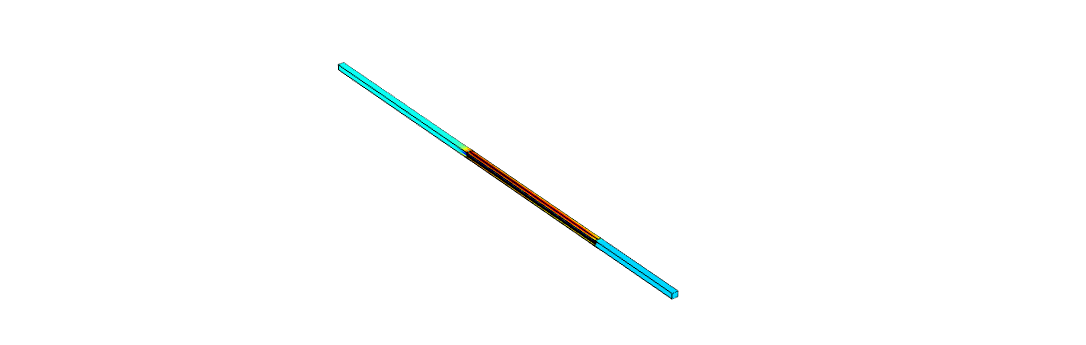
\includegraphics[width=0.8\textwidth]{00_Images/00_Velocity.png}
    \caption{Overview of the supervised learning process in neural networks.}
    \label{fig:supervised_learning}
    \end{figure}

\section{Forward Propogation}
    Forward propagation is the process by which the input is passed through the neural network to obtain the output. It involves the computation of outputs at each layer of the network until the final output is achieved. The process can be described as follows:

    Given an input vector \( \mathbf{x} \), the output of the first layer is computed as:
    \begin{equation}
    \mathbf{z}^{(1)} = \mathbf{W}^{(1)} \mathbf{x} + \mathbf{b}^{(1)}
    \end{equation}
    \begin{equation}
    \mathbf{a}^{(1)} = \sigma(\mathbf{z}^{(1)})
    \end{equation}

    where \( \mathbf{W}^{(1)} \) and \( \mathbf{b}^{(1)} \) are the weights and biases of the first layer, \( \mathbf{z}^{(1)} \) is the linear combination of inputs and weights, and \( \sigma \) is the activation function.

    This process is repeated for each subsequent layer. For the \( l \)-th layer, the computations are:
    \begin{equation}
    \mathbf{z}^{(l)} = \mathbf{W}^{(l)} \mathbf{a}^{(l-1)} + \mathbf{b}^{(l)}
    \end{equation}
    \begin{equation}
    \mathbf{a}^{(l)} = \sigma(\mathbf{z}^{(l)})
    \end{equation}

    Finally, the output of the network is obtained:
    \begin{equation}
    \hat{y} = \mathbf{a}^{(L)}
    \end{equation}

    where \( L \) is the number of layers in the network.

    \begin{figure}[h]
        \centering
        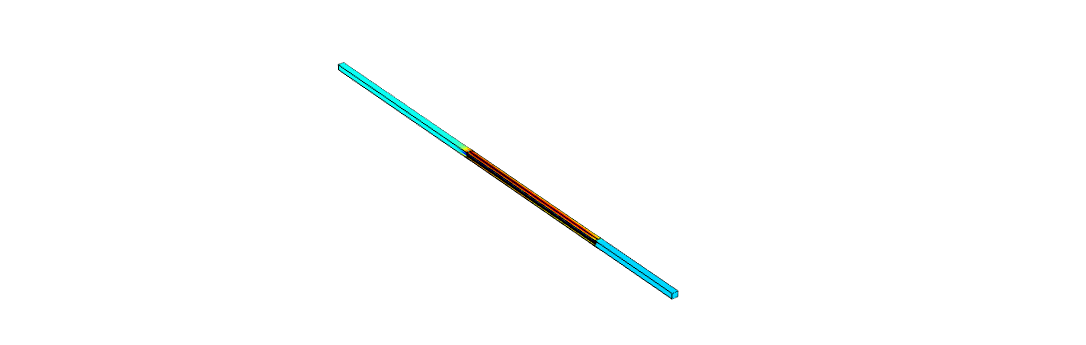
\includegraphics[width=0.8\textwidth]{00_Images/00_Velocity.png}
        \caption{Forward propagation through a neural network.}
        \label{fig:forward_propagation}
    \end{figure}

        \subsection{Activation Functions}

            Activation functions introduce non-linearity into the neural network, allowing it to learn complex patterns. Common activation functions include:

            \subsubsection{Sigmoid}

                The sigmoid function is defined as:
                \begin{equation}
                \sigma(z) = \frac{1}{1 + e^{-z}}
                \end{equation}
                It maps any real-valued number into the range (0, 1).

            \subsubsection{Hyperbolic Tangent (Tanh)}

                The tanh function is defined as:
                \begin{equation}
                \sigma(z) = \tanh(z) = \frac{e^z - e^{-z}}{e^z + e^{-z}}
                \end{equation}
                It maps any real-valued number into the range (-1, 1).

            \subsubsection{Rectified Linear Unit (ReLU)}

                The ReLU function is defined as:
                \begin{equation}
                \sigma(z) = \max(0, z)
                \end{equation}
                It outputs the input directly if it is positive; otherwise, it outputs zero.

            \subsubsection{Leaky ReLU}

                The Leaky ReLU function is defined as:
                \begin{equation}
                \sigma(z) = \begin{cases}
                z & \text{if } z \geq 0 \\
                \alpha z & \text{if } z < 0
                \end{cases}
                \end{equation}
                where \( \alpha \) is a small constant.

            \begin{figure}[h]
                \centering
                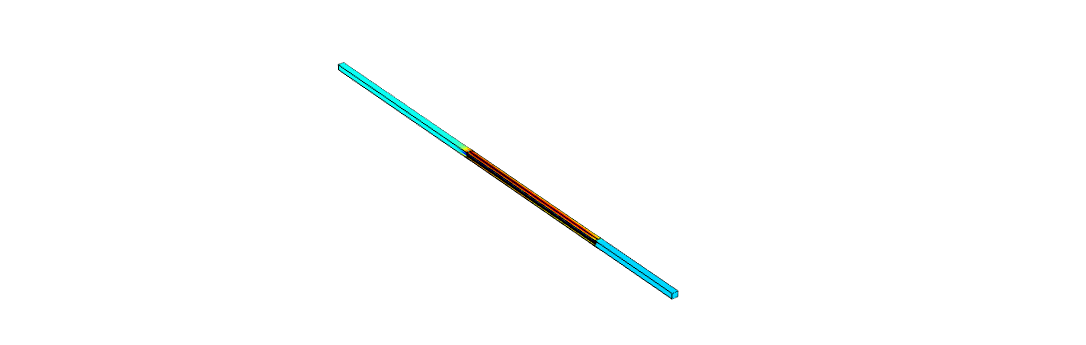
\includegraphics[width=0.8\textwidth]{00_Images/00_Velocity.png}
                \caption{Common activation functions used in neural networks.}
                \label{fig:activation_functions}
            \end{figure}

\section{Backward Propagation}

    Backward propagation, or backpropagation, is the process by which neural networks update their weights and biases to minimize the loss function. It involves calculating the gradient of the loss function with respect to each weight by the chain rule, iterating backward from the output layer to the input layer. The main steps are as follows:
    
    \begin{enumerate}
        \item \textbf{Compute the loss}: Calculate the loss \( \mathcal{L} \) between the predicted output \( \hat{y} \) and the actual output \( y \).
        \item \textbf{Calculate the gradient of the loss with respect to the output layer}: For the output layer, compute the gradient of the loss with respect to the activations.
        \item \textbf{Propagate the gradient backward through the network}: Use the chain rule to compute the gradient of the loss with respect to the weights and biases of each layer.
        \item \textbf{Update the weights and biases}: Use the gradients to update the weights and biases in a direction that reduces the loss.
    \end{enumerate}
    
    Mathematically, the gradient of the loss \( \mathcal{L} \) with respect to the weights \( \mathbf{W}^{(l)} \) and biases \( \mathbf{b}^{(l)} \) in layer \( l \) is computed as:
    
    \begin{equation}
    \frac{\partial \mathcal{L}}{\partial \mathbf{W}^{(l)}} = \delta^{(l)} \mathbf{a}^{(l-1)} 
    \end{equation}
    
    \begin{equation}
    \frac{\partial \mathcal{L}}{\partial \mathbf{b}^{(l)}} = \delta^{(l)}
    \end{equation}
    
    where \( \delta^{(l)} \) is the error term for layer \( l \) and \( \mathbf{a}^{(l-1)} \) is the activation of the previous layer.
    
    The error term \( \delta^{(l)} \) is computed as:
    
    \begin{equation}
    \delta^{(l)} = \begin{cases} 
    (\mathbf{a}^{(L)} - y) \odot \sigma'(\mathbf{z}^{(L)}) & \text{for the output layer} \\
    (\mathbf{W}^{(l+1)})^T \delta^{(l+1)} \odot \sigma'(\mathbf{z}^{(l)}) & \text{for hidden layers}
    \end{cases}
    \end{equation}
    
    where \( \odot \) denotes the element-wise multiplication and \( \sigma' \) is the derivative of the activation function.
    
    \subsection{Loss Functions}
    
        Loss functions, also known as cost functions, measure how well the neural network's predictions match the actual target values. Common loss functions include:
    
        \subsubsection{Mean Squared Error (MSE)}
    
            The Mean Squared Error is used for regression tasks and is defined as:
    
            \begin{equation}
            \mathcal{L}_{\text{MSE}} = \frac{1}{n} \sum_{i=1}^n (\hat{y}_i - y_i)^2
            \end{equation}
            
            \begin{figure}[h]
                \centering
                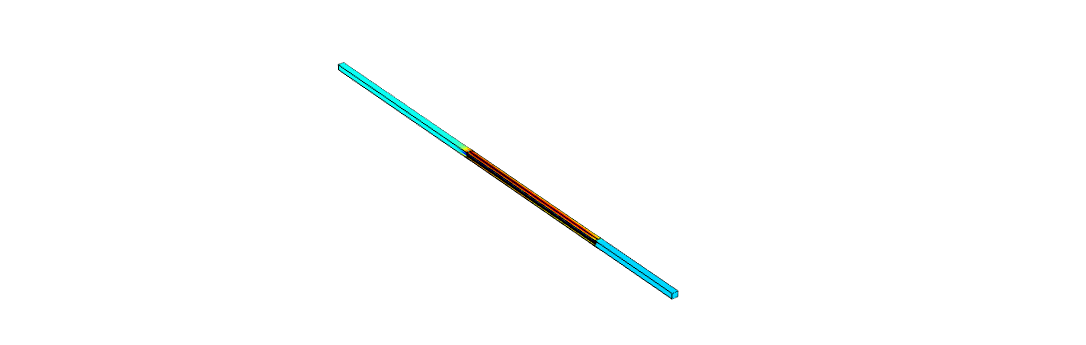
\includegraphics[width=0.8\textwidth]{00_Images/00_Velocity.png}
                \caption{Illustration of common loss functions.}
                \label{fig:loss_functions}
            \end{figure}
    
    \subsection{Methods to Update Weights}
    
        Updating the weights and biases of a neural network is a crucial part of the training process. Various methods can be employed to perform these updates:
    
        \subsubsection{Stochastic Gradient Descent (SGD)}
    
            SGD updates the weights using a single training example at a time:
    
            \begin{equation}
            \mathbf{W} \leftarrow \mathbf{W} - \eta \frac{\partial \mathcal{L}}{\partial \mathbf{W}}
            \end{equation}
    
            where \( \eta \) is the learning rate.
    
        \subsubsection{Batch Gradient Descent}
    
            Batch Gradient Descent computes the gradient using the entire training dataset:
            
            \begin{equation}
            \mathbf{W} \leftarrow \mathbf{W} - \eta \frac{1}{n} \sum_{i=1}^n \frac{\partial \mathcal{L}_i}{\partial \mathbf{W}}
            \end{equation}
    
        \subsubsection{Mini-Batch Gradient Descent}
    
            Mini-Batch Gradient Descent is a compromise between SGD and Batch Gradient Descent. It uses a small random subset (mini-batch) of the training data to compute the gradient:
    
            \begin{equation}
            \mathbf{W} \leftarrow \mathbf{W} - \eta \frac{1}{m} \sum_{i=1}^m \frac{\partial \mathcal{L}_i}{\partial \mathbf{W}}
            \end{equation}
    
            where \( m \) is the mini-batch size.
    
            \subsubsection{Adaptive Methods}
    
                Adaptive methods like AdaGrad, RMSProp, and Adam adjust the learning rate based on the history of the gradients. For example, the Adam optimization algorithm updates the weights as follows:
                
                \begin{equation}
                \mathbf{m}_t = \beta_1 \mathbf{m}_{t-1} + (1 - \beta_1) \frac{\partial \mathcal{L}}{\partial \mathbf{W}}
                \end{equation}
                
                \begin{equation}
                \mathbf{v}_t = \beta_2 \mathbf{v}_{t-1} + (1 - \beta_2) \left( \frac{\partial \mathcal{L}}{\partial \mathbf{W}} \right)^2
                \end{equation}
                
                \begin{equation}
                \hat{\mathbf{m}}_t = \frac{\mathbf{m}_t}{1 - \beta_1^t}
                \end{equation}
                
                \begin{equation}
                \hat{\mathbf{v}}_t = \frac{\mathbf{v}_t}{1 - \beta_2^t}
                \end{equation}
                
                \begin{equation}
                \mathbf{W} \leftarrow \mathbf{W} - \eta \frac{\hat{\mathbf{m}}_t}{\sqrt{\hat{\mathbf{v}}_t} + \epsilon}
                \end{equation}
                
                where \( \beta_1 \) and \( \beta_2 \) are hyperparameters, \( \mathbf{m}_t \) and \( \mathbf{v}_t \) are the first and second moment estimates, and \( \epsilon \) is a small constant.
                
            \begin{figure}[h]
                \centering
                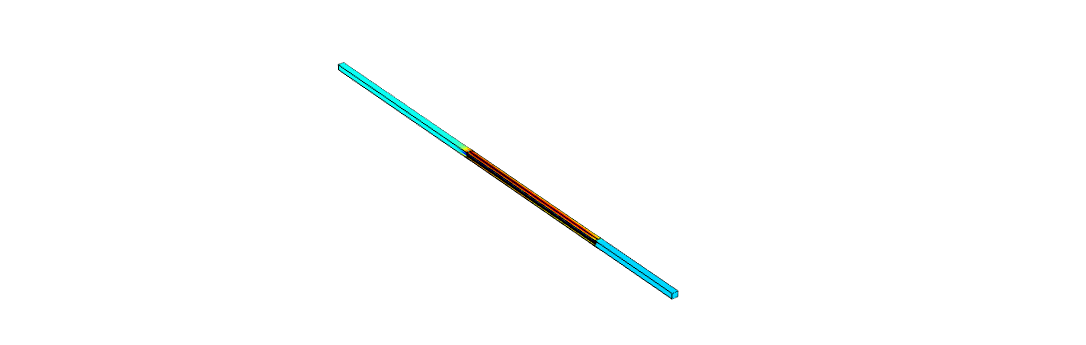
\includegraphics[width=0.8\textwidth]{00_Images/00_Velocity.png}
                \caption{Comparison of different methods to update weights.}
                \label{fig:update_methods}
            \end{figure}

\section{Hyperparameters}

    Hyperparameters are parameters whose values are set before the learning process begins. Unlike model parameters, which are learned during training, hyperparameters control the training process and influence the performance of the neural network. Common hyperparameters include learning rate, batch size, number of epochs, network architecture, activation functions, weight initialization, dropout rate, and regularization parameters.

    \subsection{Common Hyperparameters}

        \subsubsection{Learning Rate}

            The learning rate \( \eta \) controls the size of the steps taken during gradient descent to update the weights. A smaller learning rate can lead to more precise convergence but slower training, while a larger learning rate can speed up training but might overshoot the optimal solution.

        \subsubsection{Batch Size}

            Batch size determines the number of training examples used to calculate the gradient in one forward/backward pass. It influences the stability and speed of the training process. Common choices are small (stochastic gradient descent), large (batch gradient descent), or in between (mini-batch gradient descent).

        \subsubsection{Number of Epochs}

            The number of epochs defines how many times the entire training dataset passes through the network. More epochs typically improve learning, but excessive epochs can lead to overfitting.

        \subsubsection{Network Architecture}

            Network architecture includes the number of layers, the number of neurons per layer, and the type of layers used (e.g., dense, convolutional, recurrent). These choices significantly impact the capacity and capability of the network.

        \subsubsection{Activation Functions}

            Different activation functions (e.g., Sigmoid, Tanh, ReLU) can be used in different layers of the network. The choice of activation function affects the network's ability to capture non-linear patterns.

        \subsubsection{Weight Initialization}

            Weight initialization affects the starting point of the training process. Common initialization methods include random initialization, Xavier initialization, and He initialization, each suitable for different types of activation functions.

        \subsubsection{Dropout Rate}

            Dropout is a regularization technique where a fraction of neurons is randomly set to zero during training. The dropout rate controls this fraction and helps prevent overfitting by promoting the independence of neurons.

        \subsubsection{Regularization Parameters}

            Regularization parameters, such as L1 and L2 regularization, add a penalty to the loss function to constrain the model complexity. They help in preventing overfitting by discouraging overly complex models.

    \begin{figure}[h]
        \centering
        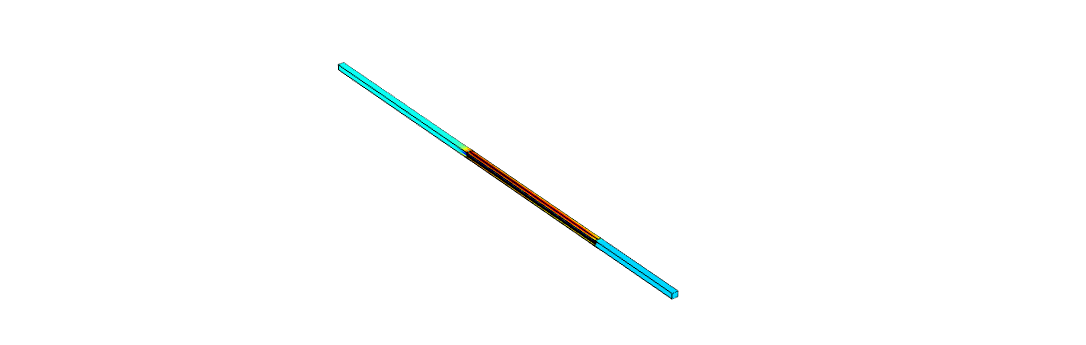
\includegraphics[width=0.8\textwidth]{00_Images/00_Velocity.png}
        \caption{Overview of common hyperparameters in neural networks.}
        \label{fig:hyperparameters}
    \end{figure}

    \subsection{Hyperparameter Optimization}

        Hyperparameter optimization involves finding the optimal set of hyperparameters that result in the best performance of the neural network. Common methods for hyperparameter optimization include:

        \subsubsection{Grid Search}

            Grid search involves specifying a set of values for each hyperparameter and training the model on all possible combinations of these values. It is computationally expensive but exhaustive.

            \begin{equation}
            \text{Optimal Hyperparameters} = \arg \min_{\eta, \text{batch size}, \ldots} \text{Validation Loss}
            \end{equation}

        \subsubsection{Random Search}

            Random search samples random combinations of hyperparameters from a predefined distribution. It is often more efficient than grid search and can find good hyperparameters with fewer iterations.

            \begin{equation}
            \text{Optimal Hyperparameters} = \arg \min_{\eta, \text{batch size}, \ldots} \text{Validation Loss}
            \end{equation}

        \subsubsection{Bayesian Optimization}

            Bayesian optimization builds a probabilistic model of the objective function and uses it to select the most promising hyperparameters to evaluate next. It is more sophisticated and can find optimal hyperparameters more efficiently.

            \begin{equation}
            \text{Optimal Hyperparameters} = \arg \max_{\eta, \text{batch size}, \ldots} P(\text{Low Validation Loss} \mid \eta, \text{batch size}, \ldots)
            \end{equation}

        \subsubsection{Hyperband}

            Hyperband is a method that combines random search with early stopping. It evaluates many configurations with a small number of iterations and progressively increases the budget for the most promising configurations.

            \begin{equation}
            \text{Optimal Hyperparameters} = \arg \min_{\eta, \text{batch size}, \ldots} \text{Validation Loss}
            \end{equation}

    \begin{figure}[h]
        \centering
        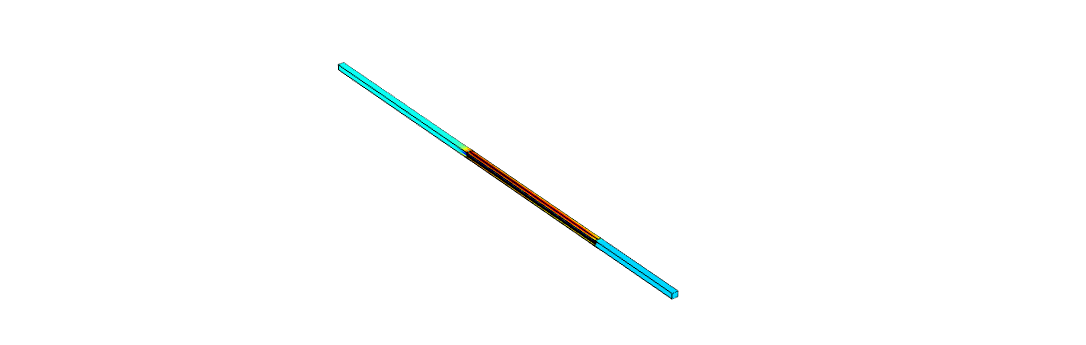
\includegraphics[width=0.8\textwidth]{00_Images/00_Velocity.png}
        \caption{Comparison of different hyperparameter optimization methods.}
        \label{fig:hyperparameter_optimization}
    \end{figure}